\documentclass[a4paper,11pt]{article}
\usepackage[utf8]{inputenc} % encodage du fichier
\usepackage[french]{babel} % document en francais
\usepackage[T1]{fontenc} % pour les caracteres accentues
\usepackage{amssymb} % Pour le symbole \nrightarrow
\usepackage{graphicx}
\usepackage[french]{algorithm2e}


\setlength{\oddsidemargin}{-10pt} % Marge gauche sur pages impaires
\setlength{\textwidth}{490pt} % Largeur de la zone de texte (17cm)
\setlength{\headheight}{-25pt} % Haut de page
\setlength{\headsep}{20pt} % Entre le haut de page et le texte


\begin{document}
\fontfamily{lmr}
\fontseries{m}
\fontsize{14pt}{18pt}
\selectfont


\section{Partie Électronique}

\subsection{Schéma Électrique}

\begin{table}[!h]
    \begin{center}
        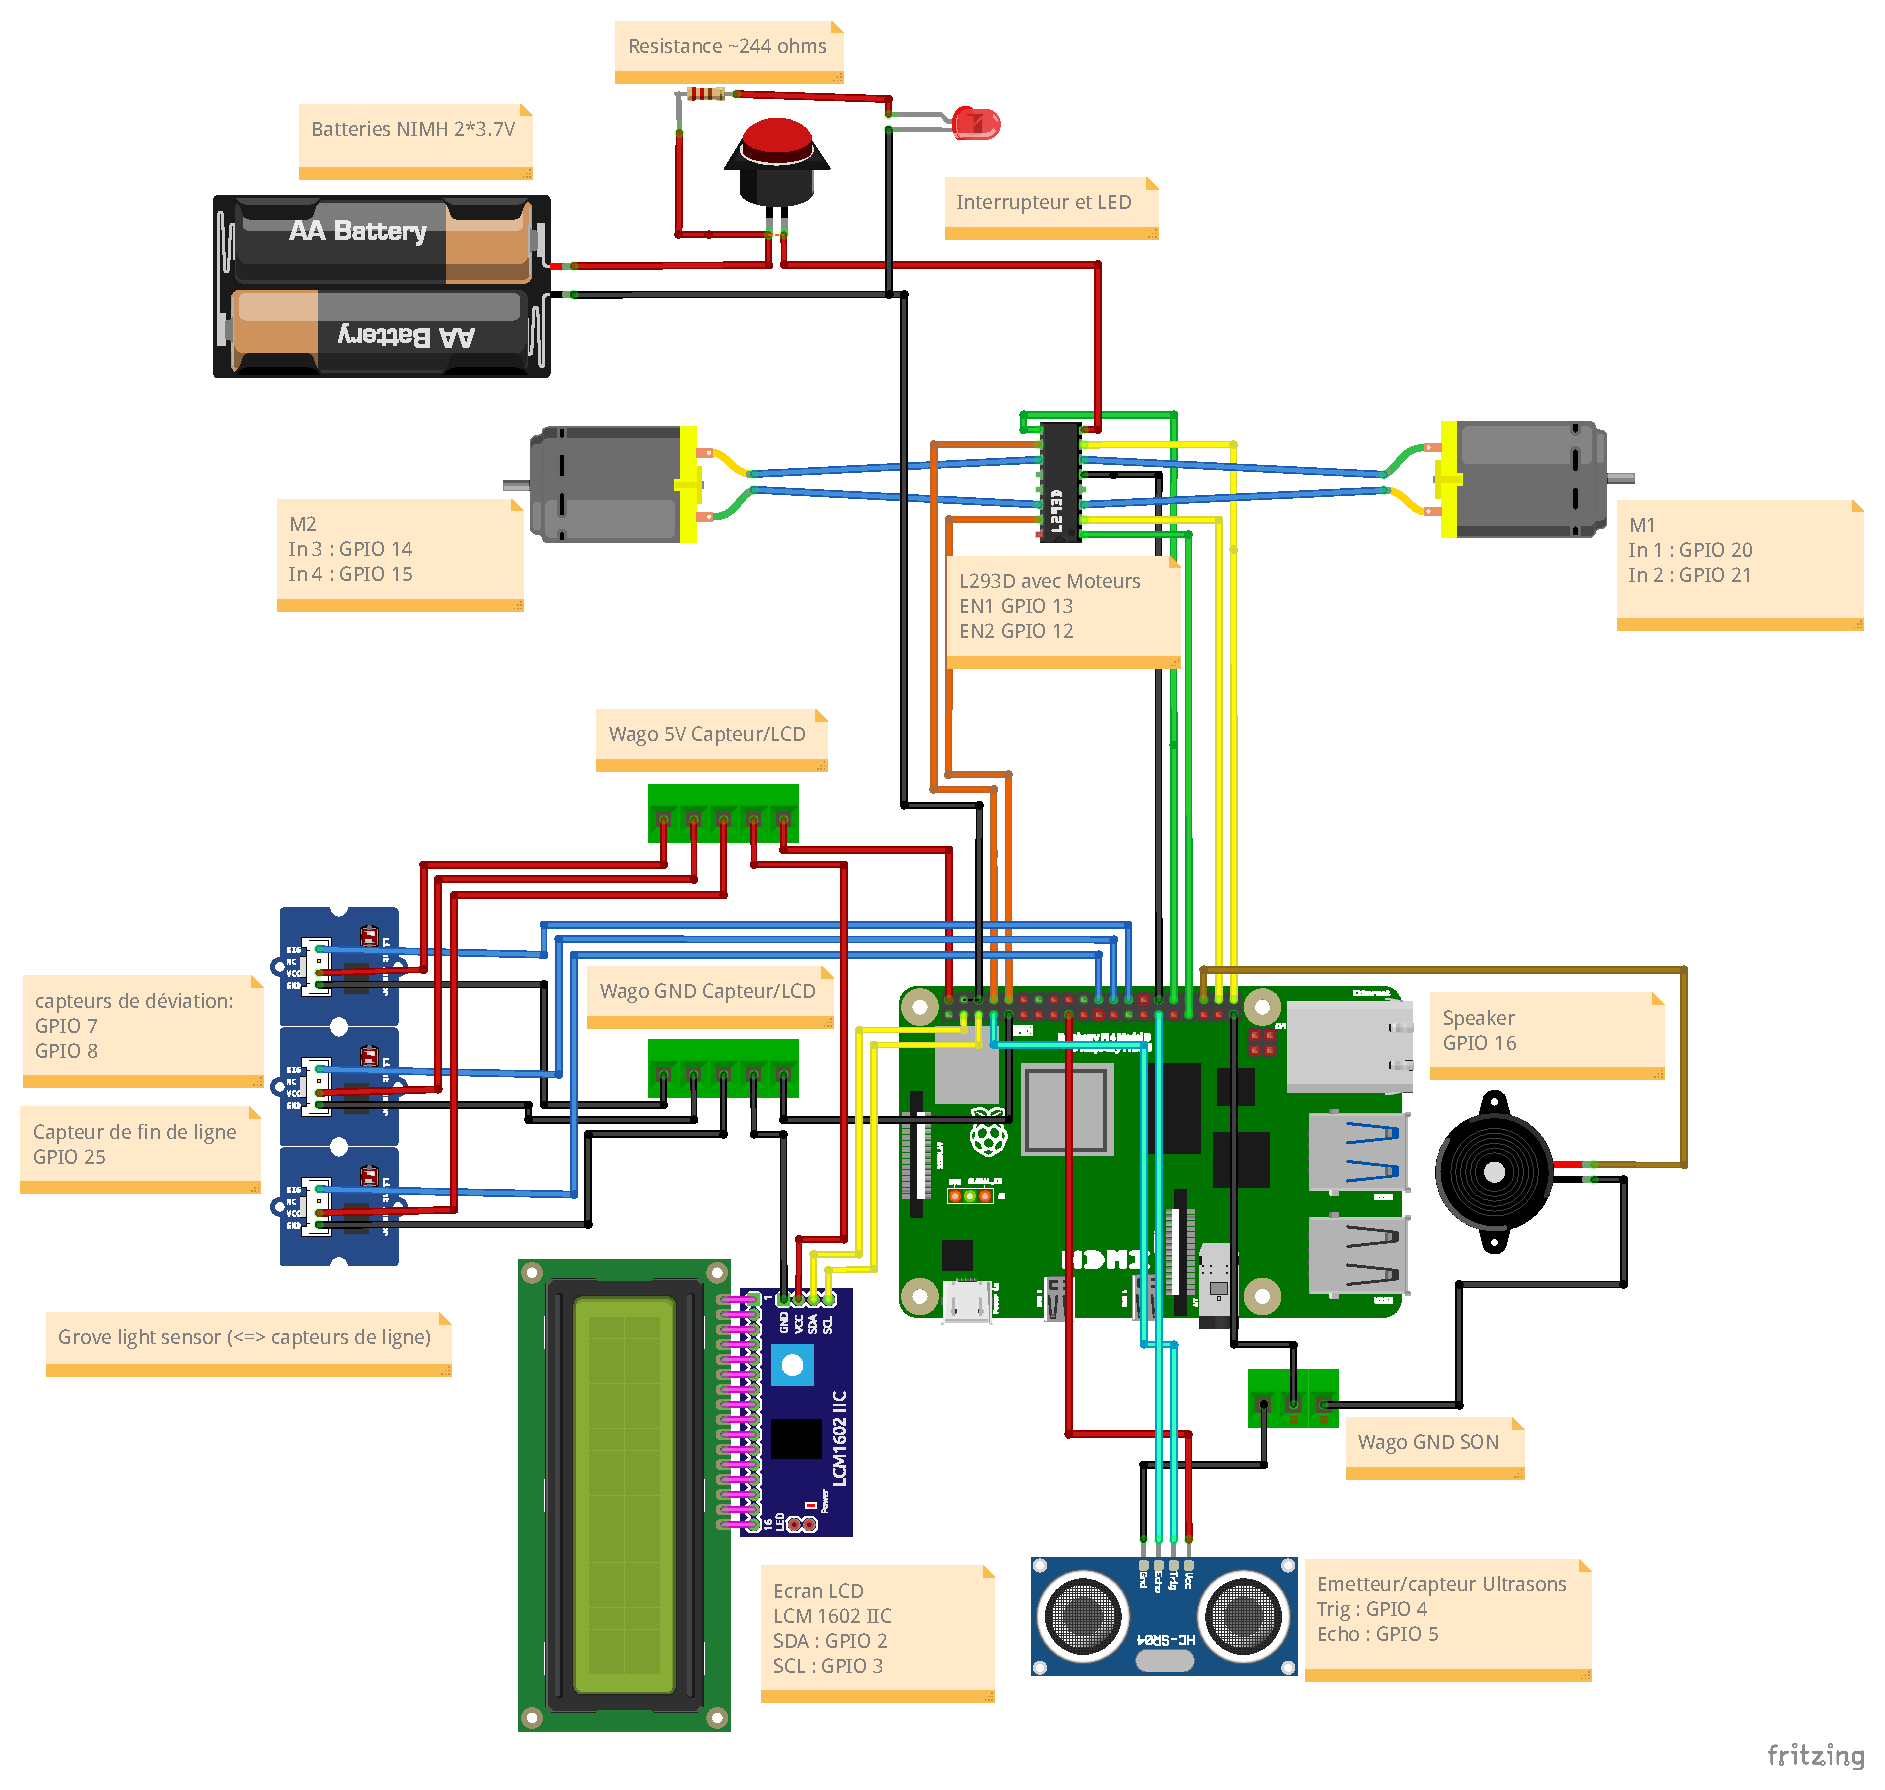
\includegraphics[width = 17cm]{figures/ElectricScheme_PISmartRobot.pdf}
    \end{center}
    \caption{Schéma Électrique du Robot}
\end{table}
\newpage

Nous avons séparé le câblage en trois pôles:
\begin{itemize}
    \item Un pôle Son
    \item Un pôle Vision
    \item Un pôle Moteur
\end{itemize}

Le premier comprend le système émetteur/récepteur d'ultrasons et le buzzer.
Un $wago$ est utilisé pour centraliser le GROUND mais les deux dispositifs sont alimenté directement sur la raspBerry 

\subsection{Positionnement des capteurs}

Nous avons pris la décision de placer trois capteurs détecteurs de ligne sur notre robot. 
Cette décision, nous avons pris du temps à la prendre et en comparant avec d'autres groupes, on remarque que beaucoup ont pris des décisions différentes.

Pourquoi trois capteurs, et quels sont leur rôle ?
Un capteur au centre (dans le trou à l'avant centre du châssis) et les deux autres à l'avant et dirigé vers les côtés.
Le capteur au centre a un rôle de contrôle: "Suis-je sur la ligne ?". Si le robot est bien sur la ligne, aucun soucis.
Sinon, les deux autres capteurs vont nous aider à savoir dans quelle situation le robot se trouve:
\begin{itemize}
    \item Cas "classique": CPTR\_estSurLaLigne
     
    le robot est sur la ligne, sur une ligne droite. Dans ce cas le capteur central est à l'état 1 et les deux capteurs extérieurs à l'état 0. Ce qui donne:

        0   1   0
    \item Intersection: CPTR\_estSurUneIntersection
    
    le robot est sur la ligne et arrive sur un virage à droite:
        
        0   1   1
    
    OU le robot est sur la ligne et arrive sur un virage à gauche:
    
        1   1   0
    
    OU le robot est sur la ligne et arrive sur une intersection (en T ou en croix)
    
        1   1   1
    \item Trop à gauche: CPTR\_estTropAGauche
    
    le robot dévie vers la gauche en ligne droite:
    
        0   0   1
    \item Trop à droite: CPTR\_estTropADroite
    
    le robot dévie vers la droite en ligne droite:
    
        1   0   0
\end{itemize}

Nous avons utilisé cette distinction de cas pour la conception des fonctions liées à l'avancement du robot dans le labyrinthe.

\subsection{Algorithme de déplacement}

\noindent\textbf{procedure} ROBOT\_evolutionRobot ()

\begin{tabular}{ll}
    \textbf{Déclaration:} & prochaineAction: \textbf{Chaine de caractères}\\
     & etat: \textbf{ROBOT\_EtatDAvancement}\\
\end{tabular}

\noindent\textbf{début}

    \begin{algorithm}[H]
        etat $\leftarrow$ Avancer\\
        \Tq{prochaineAction $\neq$ FIN}{
            \textbf{lire} (prochaineAction)\\
            \Suivant{etat}{
                \Cas{Avancer}{ROBOT\_avancer (etat)}
                \Cas{Intersection}{tourner (etat)}
                \Cas{Urgence}{ROBOT\_urgence ()}
                }
        }
    \end{algorithm}

    \noindent\textbf{fin}
\begin{center}
    \textit{Algorithme de ROBOT\_evolutionRobot}
\end{center}

Pour élaborer l'algorithme de déplacement du robot nous avons considérer qu'il pouvait se retrouver dans 4 états différents:
\begin{itemize}
    \item En avancée
    \item Sur une intersection
    \item Situation d'urgence
    \item Sorti du labyrinthe
\end{itemize} 

Nous avons donc une variable $etat$ du type \textbf{EtatDAvancement} qui est mise à jour à chaque tour d'une boucle qui ne s'arrête que lorsque la suite d'ordre que nous lui fournissons s'achève.
Selon la valeur de cette variable $etat$, différentes fonctions sont appelées afin de faire évoluer le Robot.

La première est la fonction ROBOT\_avancer, qui met les moteurs en marche avant et qui adapte la trajectoire du robot grâce aux capteurs.

Ensuite, la fonction ROBOT\_intersection agit selon l'ordre lu par l'algorithme principal. Elle fait tourner le Robot à droite ou à gauche ou bien le fait continuer tout droit.
Le Robot effectue un virage sur place, nous avons donc paramétré un temps d'attente afin de positionner correctement le centre de rotation du robot sur l'intersection.

La fonction, ROBOT\_urgence, est la fonction qui est appelée lorsqu'un obstacle est détecté. Son rôle est d'arrêter les moteurs et d'allumer le buzzer.

\subsection{Problèmes recontrés}

Pendant une grande partie du projet, nous avions le sentiment d'avoir une longueur de retard sur les autres groupes à propos de la partie électronique. 
Ce retard était dû aux nombreuses discussions que nous avions eu en amont sur la conception du Robot.
Nous avons discuté du nombre de capteurs, de la position des moteurs et d'autres dispositifs pendant plusieurs séances avant de commencer à percer et à souder.
Au final, cela ne nous a pas desservi; effectivement, après le montage, tous le câblage rentrait parfaitement dans le châssis et la plupart des composants ont fonctionné du premier coup.
De plus, la plupart des erreurs rencontrées venaient des codes utilisés.

Cependant, lors de nos premiers esssais, les moteurs ne répondaient pas. C'était une simple erreur de câblage sans gravité (aucun matériel n'a été dégradé), 
mais avec la fatigue, nous avons mal vérifié l'ensemble des connectiques et le problème ne fût résolu que lors de la séance d'essais suivante.

Avec ce retard accumulé, nous avons manqué de temps pour les derniers réglages, c'est pourquoi un dernier bug subsistait lors de la présentation du Robot.

Une voix d'amélioration de notre méthode de travail serait de définir un protocole à suivre qui aiderait à revoir l'ensemble des éléments à l'origine d'un potentiel problème rencontré.
Avec une telle méthode, nous aurions peut-être perdu moins de temps à chercher où étaient nos erreurs.

\subsection{}
\end{document}